
\documentclass[10pt,conference]{IEEEtran}

\usepackage{color}
\usepackage{url}
\usepackage{graphicx}
\usepackage{cite}
\usepackage{amsmath}
\usepackage{listings}
\definecolor{light-gray}{gray}{0.80}
%\usepackage[center]{caption}
\DeclareMathSizes{7}{7}{7}{7}
\usepackage{authblk}
\begin{document}
\title{Behavioral Analysis of the Agent-Based Community Grid Solution for the Large Hadron Collider beauty Experiment}
\author[1,3]{Daniela Remenska}
\author[2]{Tim A.C. Willemse}
\author[1]{Henri Bal}
\author[1]{Kees Verstoep}
\author[1]{Wan Fokkink}
\author[3]{Jeff Templon}

\affil[1]{Dept. of Computer Science, VU University Amsterdam, The Netherlands}
\affil[2]{Dept. of Computer Science, TU Eindhoven, The Netherlands}
\affil[3]{NIKHEF, Amsterdam, The Netherlands}

\maketitle

\begin{abstract}
DIRAC (Distributed Infrastructure with Remote Agent Control) is the Grid
solution designed to support production activities as well as user data analysis
for the Large Hadron Collider beauty experiment. It consists of cooperating
distributed services and a plethora of light-weight agents delivering the
workload to the Grid resources.  Services accept requests from agents and
running jobs, while agents actively fulfill specific goals. Services maintain
database back-ends to store dynamic state information of entities such as jobs,
queues, or staging requests. Agents continuously check for changes in the
service states, and react to these accordingly. The logic of each agent is
rather simple; the main source of complexity lies in their cooperation. These
agents run concurrently, and communicate using the services' databases as a
shared memory for synchronizing the state transitions. Despite the effort
invested in making DIRAC reliable, entities occasionally get into inconsistent
states. Tracing and fixing such behaviors is difficult, given the inherent
parallelism among the distributed components and the size of the
implementation.

In this paper we present an analysis of DIRAC with mCRL2, process algebra with
data. We have reverse engineered two critical and related DIRAC subsystems, and
subsequently modeled their behavior with the mCRL2 toolset. This enabled us to
easily locate race conditions and livelocks which were confirmed to occur in the
real system. We further formalized and verified several behavioral properties of
the two modeled subsystems.

\textbf{Keywords:} DIRAC, service-oriented architecture, agents, stager,
mCRL2,  model checking,  process algebra

\end{abstract}


\section{Introduction}

The Large Hadron Collider beauty (LHCb) experiment \cite{LHCb} is one of the
four large
experiments conducted on the Large Hadron Collider (LHC) accelerator, built by
the European Organization for Nuclear Research (CERN). Immense amounts of data
are produced at the LHC accelerator, and subsequently processed by physics
groups and individuals worldwide. The sheer size of the experiment is the
motivation behind the adoption of the Grid computing paradigm. The Grid storage
and computing resources for the LHCb experiment are distributed across several
institutes in Europe. To cope with the complexity of processing the vast amount
of data, a complete Grid solution, called DIRAC (Distributed Infrastructure with
Remote Agent Control) \cite{DIRAC_CommGridSolution},
\cite{DIRAC_ReliableDataMaangement}, has been designed and developed for the
LHCb
community.

DIRAC forms a layer between the LHCb community of users and the heterogeneous
Grid resources, in order to allow for optimal and reliable usage of these
resources. It consists of many cooperating distributed services and light-weight
agents which deliver workload to the resources. The logic of each individual
component is relatively simple; the overall system complexity emerges from the
cooperation among them. Namely, these agents run concurrently, and communicate
using the services' databases as a shared memory (blackboard paradigm \cite{IEEEexample:blackboard_systems}) for
synchronizing state transitions of various entities.

Although much effort is invested in making DIRAC reliable, entities occasionally
get into inconsistent states, leading to a potential loss of efficiency in both
resource usage and manpower. Debugging and fixing the root of such encountered
behaviors becomes a formidable mission due to multiple factors: the inherent
parallelism present among the system components deployed on different physical
machines, the size of the implementation (around 150000 lines of Python code),
and the distributed knowledge of different subsystems within the collaboration.

In this paper we propose the use of more rigorous (formal) methods for improving
software quality. Model checking \cite{ProcessesWithData} is one such technique for analysis of an
abstract model of a system, and verification of certain system properties of
interest. Unlike conventional testing, it allows full control over the execution
of parallel processes and also supports automated exhaustive state-space
exploration.

We used the mCRL2 language \cite{FormalLanguagemCRL2} and toolset \cite{mCRL2Toolset} to model the behavior of two
critical and related DIRAC components: the Workload Management (WMS) and the
Storage Management System (SMS). Based on Algebra of Communicating Processes
(ACP) \cite{process_algebra}, mCRL2 is able to deal with generic data types as well as user-defined
functions for data transformation. This makes it particularly suitable for
modeling the data manipulations made by DIRAC's agents. Visualizing the state
space and replaying scenarios with the toolkit's simulator enabled us to gain
insight into the system behavior, incrementally improve the model, and to
already detect critical race-conditions and livelocks, which were confirmed to
occur in the real system. Some of them were a result of simple coding bugs;
others unveiled more elementary design problems. We further formulated,
formalized and verified several general and application-specific properties.

The idea of modeling existing systems using 
formal techniques is as such not new. Earlier studies
(\cite{SPIN_case_study,sessionMgmtMasterThesis,desing_validation_protocols,protocol_verification_muCRL,SLAMToolkit,SlidingWindowProtocol,DHCP_SPIN}) mostly focused
on modeling and verifying hardware or communication protocols, since
the formal languages and tools at hand were not sufficiently mature
to cope with more complex data-intensive distributed systems. More
recently, success stories on modeling real-life concurrent systems with
data have been reported (\cite{CMS_LHC, Linux_driver, SystemC_processAlgebra, Java_PathFinder, ACS_mCRL2}).
In \cite{SystemC_processAlgebra} the authors have implemented a tool for automatic
translation of the SystemC language into mCRL2 statements. This greatly
simplifies the analysis, but has so far been feasible only when the
language of implementation is domain-specific, or alternatively, a
reasonably small subset of a general-purpose language is considered for
translation. The only exception in this respect is the Java Pathfinder
tool \cite{Java_PathFinder} used to find deadlocks and other behavioral properties
in Java software systems developed by NASA.

We believe that the challenges and results of this work are unique in
a number of aspects. First, to the best of our knowledge, the code-base
and the number of concurrent components engaged in providing DIRAC’s
functionality considerably outnumber previous industrial cases. Second,
the choice of Python as implementation platform has lead to prevailing
usage of dynamic structures (whose types and sizes are determined at
runtime) throughout DIRAC, challenging the transition to an abstract
formal representation. We have nevertheless established general
guidelines on extracting a model outline from the implementation. Third,
analysis of this kind is typically performed after a problem has already
surfaced in the real system, as a means to understand the events which
lead to it and test for possible solutions. We managed to stumble on an
actual bug at the same time it was observed in practice, which increased
our confidence in the soundness of the model.

The paper is organized as follows. Section 2 introduces the architecture
of DIRAC, focusing on the two subsystems chosen as case studies. Section 3 gives a brief
overview of the mCRL2 language, and describes our approach to abstracting
and modeling the behavior of these subsystems. Section 4 presents the
analysis with the mCRL2 toolset and the issues detected. Section 5
concludes and discusses future work. 

\section{DIRAC: A Community Grid Solution}
\label{sec:Section_2}
\subsection{Architecture Overview}

The development of DIRAC started in 2002 as a system for production of simulation
data that would serve to verify theory, aspects of the LHCb detector design, as
well as to optimize algorithms. It gradually evolved into a complete community
Grid solution for data and job management, based on a general-purpose framework
that can be reused by other communities besides LHCb. Today, it covers all major
LHCb tasks starting with the raw data transfer from the experiment’s detector to
the Grid storage, several steps of data processing, up to the final user
analysis. Python was chosen as the implementation language, since it enables
rapid prototyping and development of new features. DIRAC follows the Service
Oriented Architecture (SOA) paradigm, accompanied by a network of lightweight
distributed agents which animate the system. Its main components are depicted in
Fig.~\ref{fig:DIRAC-Arch}. 

\begin{figure}[t]
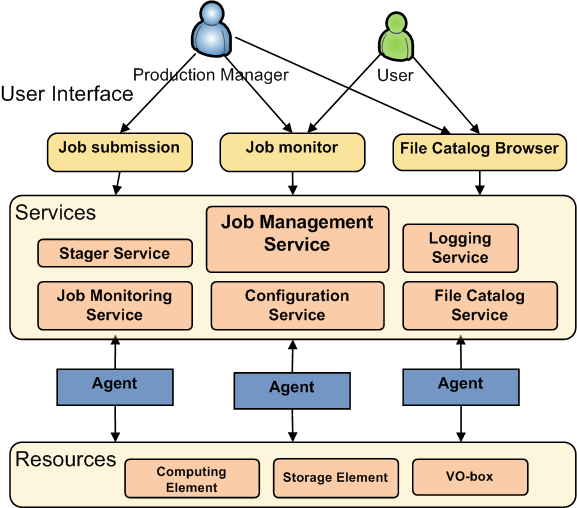
\includegraphics[width=0.85\linewidth,keepaspectratio=true]{./DIRAC_Architecture.png}
\centering
\caption{DIRAC Architecture overview}
\label{fig:DIRAC-Arch}
\end{figure}

The \textit{services} are passive components that react to requests from their clients,
possibly soliciting other services in order to fulfill the requests. They run as
permanent processes deployed on a number of high-availability hosts (VO-boxes)
at CERN, and persist the dynamic system state information in database
repositories. The user interfaces, agents or running jobs can act as clients
placing the requests to DIRAC’s services.

\textit{Agents} are active components that fulfill a limited number of specific system
functions. They can run in different environments, depending on their mission.
Some are deployed close to the corresponding services, while others run on the
Grid worker nodes.  Examples of the later are the so-called Pilot Agents, part
of the Workload Management System explained in the following section. All DIRAC
agents repeat the same logic in each iteration cycle: they observe for changes
in the service states, and react accordingly by initiating actions (like job
submission or data transfer) which may update the states of various system
entities.

\textit{Resources} are software abstractions of the underlying heterogeneous Grid
computing and storage resources allocated to LHCb, providing a uniform interface
for access. The physical resources are controlled by the site managers and made
available through middleware services such as gLite \cite{gLite}.

The DIRAC functionality is exposed to users and developers through a rich set of
command-line tools forming the DIRAC API, complemented by a Web portal for
visual monitoring the system behavior and controlling the ongoing tasks. Both
the Web and command-line \textit{interfaces} ensure secure system access using X509
certificates.

!! Mention that there are several subsystems part of DIRAC's architecture.
We focus on two related subsystems that were considered essential, yet 
are the ones where problematic state changes were most often encountered, 
and difficult to trace and correct.  

\subsection{Workload Management System}

The driving force of DIRAC is the Workload Management System (WMS). Taking into
account that the distributed computing environment is intrinsically unstable, a
\textit{Pilot Job paradigm}, illustrated in Fig.~\ref{fig:DIRAC-WMS}, was chosen as an efficient way to
implement a pull scheduling mechanism.  Pilot jobs are simply resource
reservation processes without an actual payload defined apriori. They are
submitted to the Grid worker nodes with the aim of checking the sanity of the
operational environment just before pulling and executing the real payload. This
hides the fragility of the underlying resources and increases the job success
rate, from the perspective of end users Centralized \textit{Task Queues} contain all the
pending jobs, organized in groups according to their requirements. This enables
efficient application of job priorities, enforcing faire-share policies and
quotas, which are decided within the LHCb community, without the need of any
effort from the Grid sites.  
\begin{figure}[t]
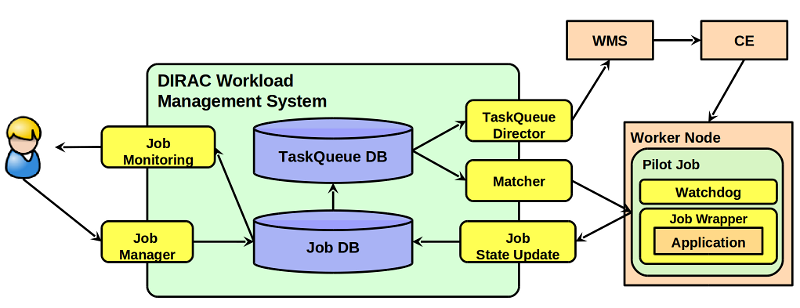
\includegraphics[width=\linewidth,keepaspectratio=true]{./DIRAC_WMS1.png}
\centering
\caption{DIRAC Workload Management System \cite{DIRAC_pilot_WMS}}
\label{fig:DIRAC-WMS}
\end{figure}
 \begin{figure}[b]
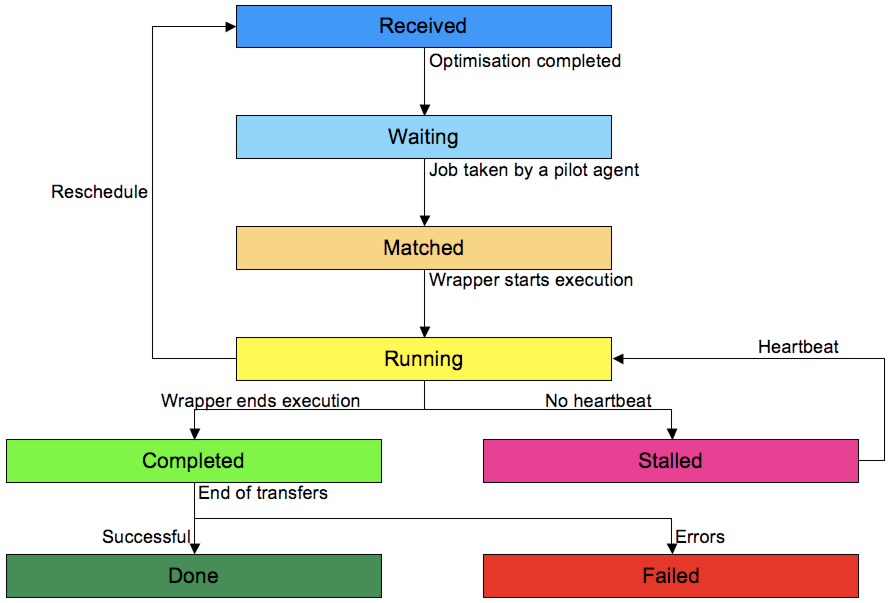
\includegraphics[width=\linewidth,keepaspectratio=true]{./dirac-primary-states.png}
\centering
\caption{Job state machine \cite{ProductionShifterGuide}}
\label{fig:DIRAC-job-state-machine}
\end{figure} 

The basic flowchart describing the evolution of a job’s states is depicted in
Fig.~\ref{fig:DIRAC-job-state-machine}. After submission through the \textit{Job Manager} (``Received''), the complete
job description is placed in the DIRAC job repository (the Job DB). Before jobs
become eligible for execution, a chain of optimizer agents check and prioritize
them in queues, utilizing the parameters information from the Job DB. \textit{The Job
Sanity Agent} can meaningfully fail jobs with impossible requirements, and
prevent unnecessary submission to the Grid resources.The \textit{Input Data Agent}
performs a resolution of possible target computing resources based on the input
data requirements. If the requested data resides on tape storage, the \textit{Job
Scheduling Agent} will pass the control to a specialized \textit{Stager} service (part of
the SMS explained in the next section), before placing the job a Task Queue
(``Waiting''). Based on the complete list of pending payloads, a specialized \textit{Task
Queue Director} submits pilots to the computing resources via the gLite WMS. After
a \textit{Matcher} service pulls the most suitable payload for a pilot (``Matched''), a \textit{Job
Wrapper} object is created on the worker node, responsible for retrieving the
input sandbox, performing software availability checks, executing the actual
payload on the worker node (``Running''), and finally uploading any output data
necessary (“Done” or ``Failed''). The wrapper can catch any failure exit state
reported by the running physics applications. At the same time, a \textit{Watchdog}
process is instantiated to monitor the behavior of the Job Wrapper and send
heartbeat signals to the monitoring service. It can also take actions in case
resources are soon to be exhausted, the payload stalls, or a management command
for killing the payload is received.

Although the Grid storage resources are limited, it is essential to keep all
data collected throughout the experiment’s run. Tape backends provide a reliable
and cheap solution for data storage. The additional workflow step 
necessary for input data files residing on tape is carried out inside the
Storage Management System (SMS).

\subsection{Storage Management System}

The DIRAC SMS provides the logic for pre-staging files from tape to a disk cache
frontend, before a job is able to process them. Smooth functioning of this
system is essential for production activities which involve reprocessing of
older data with improved physics software, and happens typically several times
per year.

A simplified view of the system is shown in  Fig.~\ref{fig:DIRAC-SMS}. The workflow is initiated
with the Job Scheduling agent detecting that a job is assigned to process files
only available on tape storage. It sends a request for staging (i.e., creating a
cached replica) to the \textit{Storage Manager Handler} service along with the
list of files and a callback method to be invoked when the request has been
processed. The Storage Management DB is immediately populated with records which
are processed by a sequence of agents in an organized fashion. The relevant
tables in the SMS DB are the \textit{Tasks} and \textit{CacheReplicas}, whose
entities maintain a state observed and updated by these agents. Tasks maintain
general information about every job requesting a service from the SMS. The
details about every file (i.e., the Storage Element where it resides, the
size, checksum, number of tasks that requested it), are kept in the CacheReplicas
table. Other auxiliary tables maintain the relationship between these entities.
\begin{figure}[t]
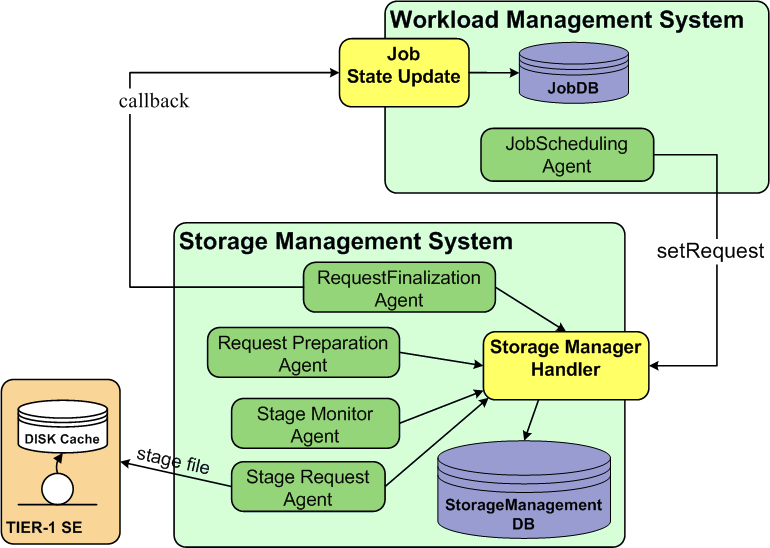
\includegraphics[width=0.9\linewidth,keepaspectratio=true]{./SMS_simplified.png}
\centering
\caption{DIRAC Storage Management System}
\label{fig:DIRAC-SMS}
\end{figure}

The processing begins with the \textit{Request Preparation Agent}. It selects all the
``New'' entries for files, checks whether they are registered in a special Logical
File Catalog (LFC), and retrieves their metadata. In case of problematic catalog
entries, it can update the status of the CacheReplicas and the related Tasks
entries to ``Failed''. For non-problematic files it carries out transition to
``Waiting''. The \textit{StageRequest Agent} is responsible for placing the actual staging
requests for all ``Waiting'' entries, via dedicated storage middleware that
communicates with the tape backends. These requests are grouped by SE prior to
submission, and carry information about the requested (pin) lifetime of the
replicas to be cached. If certain pathologies are discovered (i.e., lost,
unavailable or zero-sized files on tape), it can update the corresponding
entries to ``Failed'' in a similar manner. Otherwise, they are promoted to
``StageSubmitted''. The agent responsible for monitoring the status of submitted
requests is the \textit{StageMonitor Agent}. It achieves this by interrogating the
storage middleware to see if the ``StageSubmitted'' files are successfully
replicated on disk cache. In case of success, the CacheReplicas and their
corresponding Tasks entries are updated to ``Staged''. Various circumstances of
tape or middleware misbehavior can also fail the staging requests. The last one
in the chain is the \textit{RequestFinalization Agent}. The tasks which are in their
final states (``Staged'' or ``Failed'') are cleared from the database, and callbacks
are performed to the WMS, which effectively wakes up the corresponding jobs. If
there are no more associated tasks for particular replicas, the respective
CacheReplicas entries are also removed.

This subsystem is still in evolutionary phase. In multiple instances, tasks or
replicas have become “stuck”, effectively blocking the progress of jobs. Tracing
back the sequence of events which led to the inconsistent states is non-trivial.
To temporarily alleviate such problems, the status of these entries is typically
reset to the initial “New” state manually, so agents can re-process them from
scratch. Occasionally, error messages are reported from unsuccessful attempts of
the SMS service to update the state of a non-existent table entry.

\section{System modeling}
\subsection{The mCRL2 language and toolset}
tbw
\subsection{From DIRAC to mCRL2}

Any formal analysis uses a simplified description of the real system. Even in the 
best possible scenario, where the target implementation language and the modeling 
notation are very close (\cite{Java_PathFinder},\cite{Musuvathi04modelchecking}), 
it is practically impossible to avoid the use of abstraction to create a simplified model. 
Software implementations are large and often contain many details that can be irrelevant 
for the intended analysis. Abstraction aims at reducing
the program's state space in order to overcome the resource limitations \cite{Pelánek08fightingstate} encountered during model-checking.
Furthermore, specification languages describe \textit{what} is being done, 
abstracting away from the details of \textit{how} things are done. 
Then, the ultimate question is: \textit{how do we establish correspondence between model and code?}

High-level design documents are a good starting point, but insufficient for 
building a sound model.
In absence of more detailed up-to-date behavioral models, 
we based our models on the source code and discussions with developers.
A popular abstraction technique
for identifying code subsets (slices) that (potentially) affect particular 
variables of interest (slicing criteria) is program slicing \cite{Hatcliff99slicingsoftware}. 
It reduces the behavior of a program
by removing control statements and data structures deemed irrelevant for 
the criteria. Unfortunatelly, to the best of our knowledge, the only practical
applications of automated slicing have been
on C/C++ and Java programs.[references] Research has not yet
matured on this topic for dynamic languages, such as Python. 
Therefore, we performed the program slicing manually, relying on the Eclipse IDE for 
reverse-engineering and dependency analysis of the subsystems.

Given the reccurent invalid state transitions of entities within DIRAC, 
we considered the possible race conditions caused by multiple agents updating 
the service states to be the target of our analysis. We limit the scope
to analysis of the following entities: \textit{Tasks} (SMS), \textit{CacheReplicas} (SMS) and \textit{Jobs} (WMS).
This determines our slicing criteria. In the following, we use the SMS as a case study
for describing the established modeling guidelines. They can be 
directly applied to other DIRAC systems. First, the 
guidelines are informaly described, followed by fragments 
of the mCRL2 model to illustrate the translation.

\subsubsection{Control Abstractions}
As already explained, all agents repeat the same logic in every subsequent iteration:first they
read some entries of interest from the service database, then they process the cached data, and finally
they may write or update entries back, based on decisions from the processing step.
They can be naturally modelled as \textit{recursive processes}.
Take as an example the code snippet\footnote{This method is $\sim$100 lines of code in reality} 
in Listing~\ref{listing1}, 
from the simplest agent: the \textit{Stage Request Agent}. 
Although much of the code is omitted for clarity, the necessary parts for
ilustrating the basic idea are kept.
The first highlighted statement is the selection of all "New'' CacheReplicas
entries. What follows is retrieval of their metadata from the LFC,
external to this subsystem. Subsequently, list and dictionary manipulations
are done to group the retrieved data depending on the outcome.
Two lists of replica IDs are built before the last step: one for the problematic catalog entries,
and one for the sucesful sanity checks.
Finally, the last two highlighted code segments update the states 
of the corresponding CacheReplicas to "Failed'' and ``Waiting'' respectfully.

\definecolor{light-gray}{gray}{0.90}

\lstset{language=Python,tabsize=2,caption={Request Preparation Agent },
  stringstyle=\ttfamily,
  %basicstyle=\small,
  label=listing1,
  %frame=trbl,
  breaklines=true,
  showstringspaces=false,
  boxpos=t,
  belowcaptionskip=5pt
 }

\begin{lstlisting}[float=tp,escapechar=!,basicstyle=\ttfamily\fontsize{7}{7}\selectfont]
  def prepareNewReplicas( self ):
    """ This is the first logical task to be executed 
    """ and manages the New->Waiting transition of the Replicas
    !\colorbox{light-gray}{res = self.getNewReplicas()}!
    if not res['Value']:
      gLogger.info('There were no New replicas found')
      return res
    [...]
    # Obtain the replicas from the FileCatalog
    res = self.__getFileReplicas( fileSizes.keys() )
    if not res['OK']:
      return res
    failed.update( res['Value']['Failed'] )
    terminal = res['Value']['ZeroReplicas']
    fileReplicas = res['Value']['Replicas']
    [...]
    replicaMetadata = []
    for lfn, requestedSEs in replicas.items():
      lfnReplicas = fileReplicas[lfn]
      for requestedSE, replicaID in requestedSEs.items():
        if not requestedSE in lfnReplicas.keys():
          terminalReplicaIDs[replicaID] = "LFN not registered at requested SE"
          replicas[lfn].pop(requestedSE)
        else:
          replicaMetadata.append((replicaID, lfnReplicas[requestedSE], fileSizes[lfn]))

    # Update the states of the files in the database
    if terminalReplicaIDs:
      gLogger.info('%s replicas are terminally failed.' % len( terminalReplicaIDs ) )
      !\colorbox{light-gray}{res = self.stagerClient.}!
	    !\colorbox{light-gray}{updateReplicaFailure(terminalReplicaIDs)}!
    if replicaMetadata:
      gLogger.info('%s replica metadata to be updated.' % len( replicaMetadata ) )
      # Sets the Status='Waiting' of CacheReplicas records 
      #that are OK with catalogue checks
      !\colorbox{light-gray}{res = self.stagerClient.}!
	    !\colorbox{light-gray}{updateReplicaInformation( replicaMetadata )}!
    return S_OK()

\end{lstlisting}

The logging statements, although critical for operational matters, will
not affect the entries' states, and can be translated to \textit{silent steps} in mCRL2.
Furthermore, instead of tracing back and modeling all variables on which 
the two final lists depend, we can use nondeterminism. 
It is not known upfront which branch execution will follow
for a particular replica, as it depends on external behaviour (i.e. the interactions of the system with its environment)
However, by stubbing-out the communication with the LFC and
most of the local variable manipulations 
that follow, and replacing them with a \textit{nondeterministic choice} between the two
ultimate state updates, we can include both possibilities in the model behavior,
and still preserve correctness. Of course, depending on the context, some 
variable values cannot be ignored, in which case decisivness can be preserved
using \textit{if-then-else} mCRL2 statements. All relevant selection and update 
statements are translated into \textit{parametrized actions}.
 
\subsubsection{Data Abstractions}
The CacheReplicas entity contains more information besides the state.
Every database entry has a unique identifier, descriptive data such as 
the SE where it resides, its full path, checksum, timestamps etc. 
Model checking can only be performed on closed models, where the domains
of all variables are finite. Since we are only interested in state transitions,
we can collapse most of this descriptive data, and represent this entity as a 
\textit{custom sort} in mCRL2:
%\begin{lstlisting}[tabsize=10,basicstyle=\ttfamily\fontsize{8}{7}\selectfont]
\begin{displaymath}
\begin{align*}
sort\ CacheReplicas = \textbf{struct}\ Start?is\_start\ | \\
			  New?is\_new\ |  \\
		    Waiting?is\_waiting\ | \\
          StageSubmitted?is\_stageSubmitted\ | \\ 
		      Staged?is\_staged\ | \\
		      Failed?is\_failed\ | \\
		  Deleted?is\_deleted\ ;
\end{align*}
\end{displaymath}
%\end{lstlisting}
This defines an enumerated data type with all possible states, together with constructor and recognizer functions.
The Tasks entity is modeled in the same manner. Lists of these sorts can be easily modeled 
in mCRL2 as \begin{math}List(Tasks) \end{math} and 
\begin{math}List(CacheReplicas) \end{math}.
To define the many-to-many relationship between Tasks and CacheReplicas,
we join these data elements in a tuple:
%\begin{lstlisting}[tabsize=10,basicstyle=\ttfamily\fontsize{8}{7}\selectfont]
\begin{displaymath}sort \ Tuple = \textbf{struct}\ p(t:Nat,r:Nat,link:Bool)
\end{displaymath}
%\end{lstlisting}
The first two elements are the list positions of the Tasks and CacheReplicas
entries, while the last one indicates whether a relation between
them exists at a given moment of the system execution. The projections 
($t:Tuple\mapsto Nat$, $r:Tuple\mapsto Nat$, $link:Tuple\mapsto Bool$)
of the tuple on the individual data types are automatically defined with the above
statement.

In reality agents operate on lists of IDs corresponding to the database
entries, so functions for transforming items of type \begin{math}List(CacheReplicas)\end{math}
and \begin{math}List(Tasks)\end{math}
to a list of identifiers (i.e., positions) 
\begin{math}List(Nat)\end{math} are necessary.
One such \textit{data transformation} used in the model is the 
$t2id:List(Tasks)\times Tasks\mapsto List(Nat)$ function, which,
given an existing list of Tasks and a specific Tasks value, returns the list positions
 matching the value.
For example:
% example t2id([one,two,two,three],two)->[1,2] 
\begin{displaymath}
t2id([New,Staged,Staged,Failed],Staged)\rightarrow [1,2] 
\end{displaymath}
Another example is the 
$id2cr:List(Nat)\times Lsit(CacheReplicas)\times CacheReplicas\mapsto List(CacheReplicas)$                                                                                                
function, which can be used to update certain CacheReplicas list entries with a new value, in the following way:
\begin{displaymath}
id2cr([0,1],[Waiting,Staged,New],Failed) \\
 \rightarrow \\
\end{displaymath}
\begin{displaymath}
[Failed,Failed,New]
\end{displaymath}
These data transformations provide a natural way of modeling
the actual database operations.

The mCRL2 language does not allow global variables (or a similar construct).
Therefore, the shared database is modeled as a parametrized wrapper process
that keeps the entries in its local memory, as illustrated in Figure~\ref{fig:CRMemory}.
\begin{figure*}[!t]

$proc\ CacheReplicaMem(d:List(CacheReplicas)) = $

$\sum_{t:CacheReplicas} RPAgent\_selectCacheReplicas\_(cr2id(d,t),t).
CacheReplicaMem(d) +$

$\sum_{l:List(Nat),t:CacheReplicas} RPAgent\_prepareNewReplicas\_(l,t).CacheReplicaMem(id2cr(l,d,t))+$

$\dots\ +$ 

$\sum_{l:List(Nat),t:CacheReplicas} RFAgent\_removeReplicas\_(l,t).CacheReplicaMem(id2cr(l,d,t))+$

$CacheReplicaMem(d);$

\caption{CacheReplicas memory process}
\label{fig:CRMemory}
\end{figure*}
By means of process communication, the shared list of entries can be obtained
and changed by the agent processes. The
recursive process continously listens and responds
to requests from other processes (agents).
The summation operator allows the process to 
accept any value of the \begin{math}CacheReplicas\end{math}
and \begin{math}List(Nat)\end{math} sort passed by agents.
To ensure that such synchronous communication between the memory process and the agents
is possible, the mCRL2 \begin{math}allow\end{math}
and \begin{math}comm\end{math}
constructs are used
in the \begin{math}init\end{math}
part of the specification:

$ \Delta_{\{RPAgent\_selectCacheReplicas,
    RPAgent\_prepareNewReplicas, } $
  $    _{\dots\\, RFAgent\_removeReplicas\}} $

$ \Gamma_{\{\_RPAgent\_selectCacheReplicas|
   RPAgent\_selectCacheReplicas\_} $
  $  _{\rightarrow RPAgent\_selectCacheReplicas, } $
  $ _{\_RPAgent\_prepareNewReplicas|RPAgent\_prepareNewReplicas\_} $
  $  _{\rightarrow RPAgent\_prepareNewReplicas,\dots\\, } $
 $ _{\_RFAgent\_removeReplicas|RFAgent\_removeReplicas\_} $
  $  _{\rightarrow RFAgent\_removeReplicas\}} $
$ \\ $

To complete the picture, we give an outline of the model for the \begin{math}Request Preparation Agent\end{math}:

$ _{RPAgent = }$
	$ _{\sum_{cc:List(Nat)} \_RPAgent\_selectCacheReplicas(cc,New). }$

	$ _{((cc\neq[])\rightarrow \ (\_RPAgent\_prepareNewReplicas(cc,Failed). } $

	$_{	\sum _{tt:List(Nat)} \_RPAgent\_selectTaskReplicas(tt,cc).  }$

	$_{	((tt\neq[])\rightarrow \_RPAgent\_prepareNewReplicasT(tt,tFailed)\ \diamond \ \tau)\ + }$  

	$ _{\_RPAgent\_prepareNewReplicas(cc,Waiting))\ \diamond \ \tau) } $

$ _{.RPAgent; }$
$ \\ $

%Since the services are the frontend for all interractions with the storage,
%they essentially act as wrappers around the storage. By already modeling
%the storage as a recursive process with memory, there is no need to model them explicitely. 

Thus, so far we have established: a) a finite domain of abstract values, b) an
abstraction for mapping concrete program values to abstract ones and
c) collection of processes built from parametrized actions describing 
the behavior of the program components.
Substituting concrete operations on real data of interest
with the corresponding operations of the abstract interpretation yields 
our abstract model. Finally, the model is put together as a parallel composition of all
communicating processes.

\section{Analysis and Issues}
\label{sec:Section_4}
\section{Conclusions and Future Work}
\label{sec:Section_5}

\bibliographystyle{IEEEtran} 
\bibliography{myLibrary}

\end{document}


